\documentclass{beamer}
\usetheme{Madrid}
\usecolortheme{beaver}
\usepackage{textpos}

\title{TRIUMF nEXO SiPM Studies}
\author[]{
\includegraphics[height=2.0cm,width=2.2cm]{./EXO.png}\\ \vspace{0.5cm} \\Fabrice Reti\`{e}re\\Carl Rethmeier\\Lloyd James\\Paul Lopes Gomes\vspace{-0.5cm}}
\institute[]{
\includegraphics[height=0.8cm,width=2.5cm]{./TRIUMF.png}}
\date{\today}

\setbeamertemplate{footline}
{
  \leavevmode%
  \hbox{%
  \begin{beamercolorbox}[wd=.333333\paperwidth,ht=2.25ex,dp=1ex,right]{author in foot/foot}%
    \usebeamerfont{author in foot/foot}\insertshortauthor%~~\beamer@ifempty{\insertshortinstitute}{}{(\insertshortinstitute)}
  \end{beamercolorbox}%
  \begin{beamercolorbox}[wd=.333333\paperwidth,ht=2.25ex,dp=1ex,center]{title in foot/foot}%
    \usebeamerfont{title in foot/foot}\insertshorttitle
  \end{beamercolorbox}%
  \begin{beamercolorbox}[wd=.333333\paperwidth,ht=2.25ex,dp=1ex,right]{date in foot/head}%
    \usebeamerfont{date in foot/head}\insertshortdate{}\hspace*{2em}
    \insertframenumber{} / \inserttotalframenumber\hspace*{2ex} 
  \end{beamercolorbox}}%
  \vskip0pt%
}
\makeatother


\begin{document}

\begin{frame}
\maketitle
\end{frame}

\addtobeamertemplate{frametitle}{}{%
\begin{textblock*}{100mm}(.85\textwidth,-1cm)
\vspace{0.5mm}
\hspace{-2.5cm}

\includegraphics[height=0.8cm,width=2.5cm]{./TRIUMF.png}
\hspace{0.5cm}

\includegraphics[height=0.9cm,width=0.9cm]{./EXO.png}
\end{textblock*}}

\begin{frame}{VUV3 Breakdown Voltage}
\begin{figure}
\centering
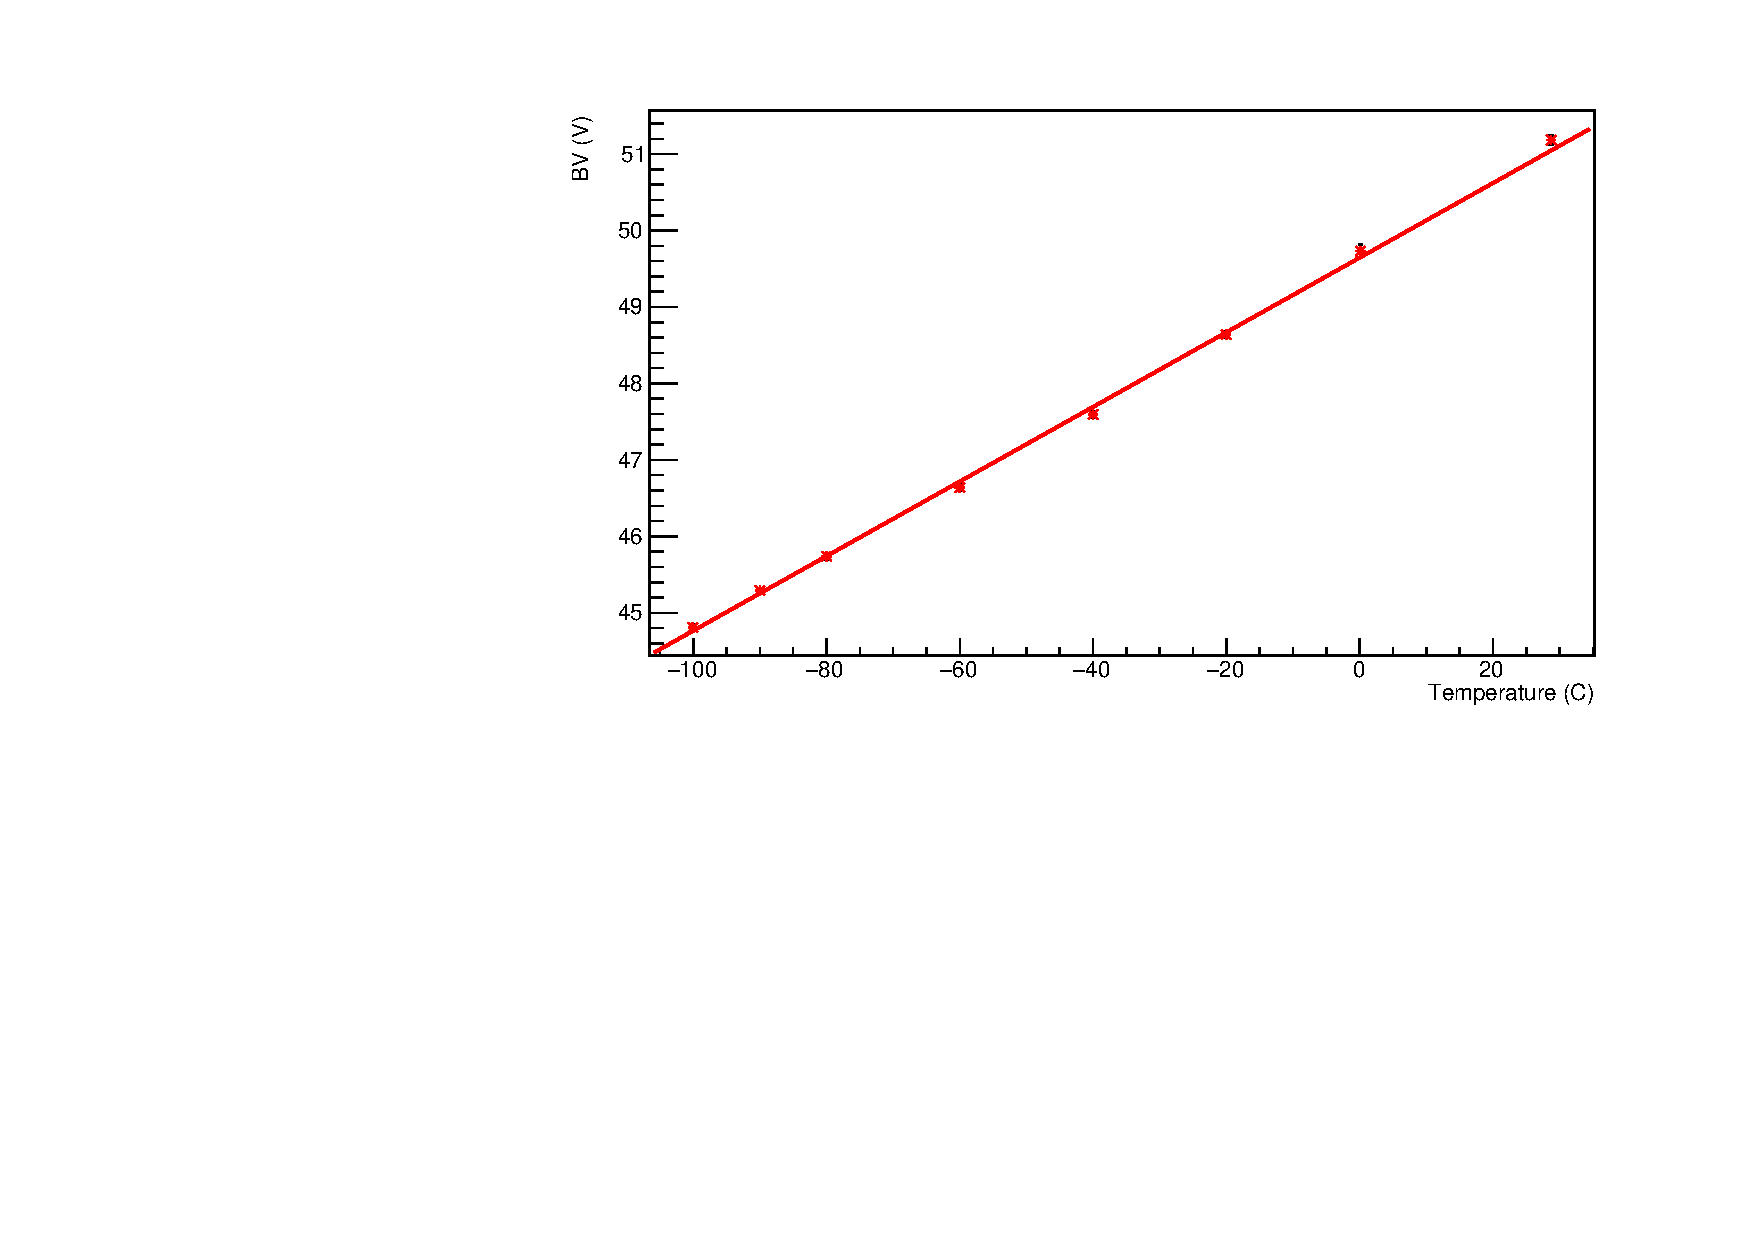
\includegraphics[height=0.5\textwidth]{Gain_Temperature.pdf}
\caption{Breakdown Voltage against Temperature for VUV3 device.}
\end{figure}
\end{frame}

\begin{frame}{Cross-talk}
\begin{figure}
\centering
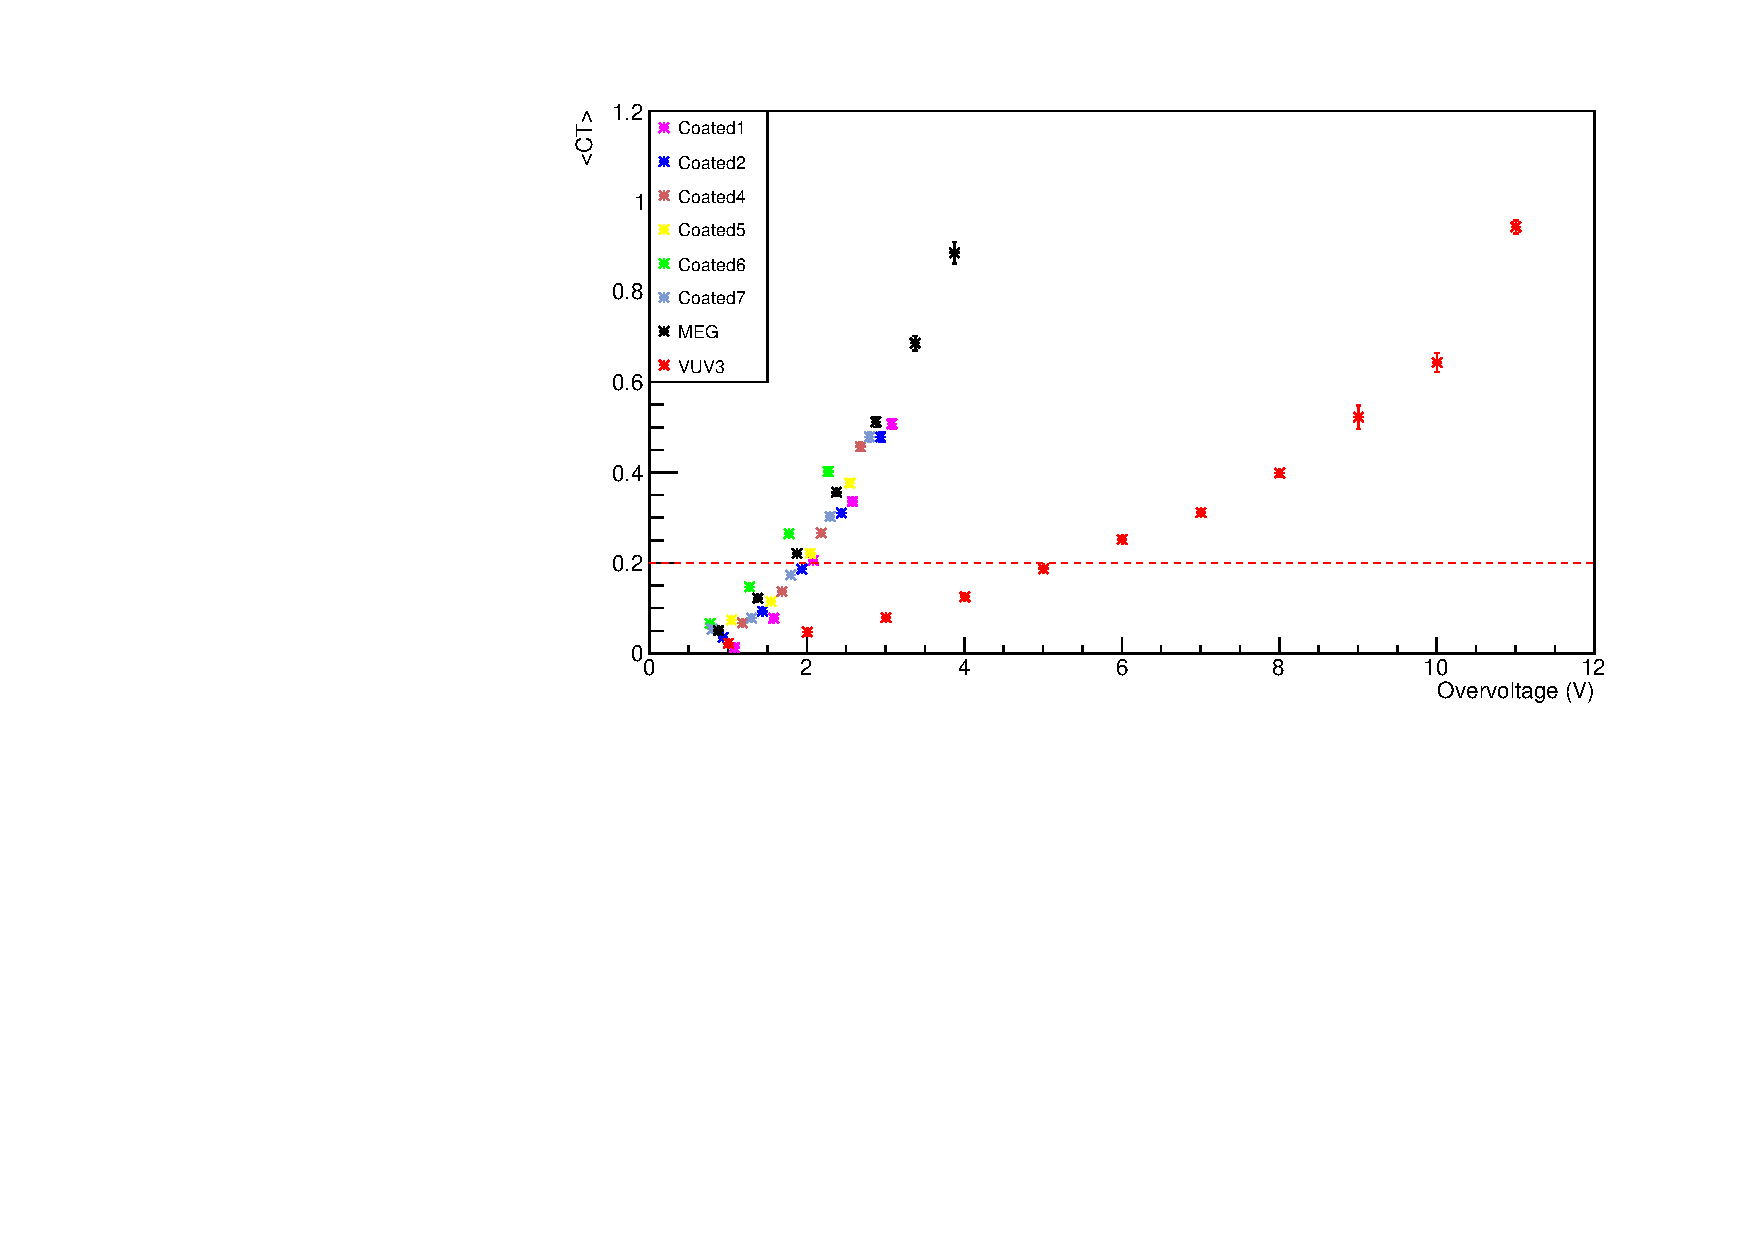
\includegraphics[height=0.5\textwidth]{CTAug7.pdf}
\caption{Crosstalk rate against overvoltage for different devices.}
\end{figure}
\end{frame}

\begin{frame}{Automation}
\begin{itemize}
Remote control of the power supply / picoammeter was implemented and interfaced with the scope DAQ software so that voltage scans can now be done automatically. 
\end{itemize}
\end{frame}

\begin{frame}{Delta-t Distribution}
\begin{figure}
\centering
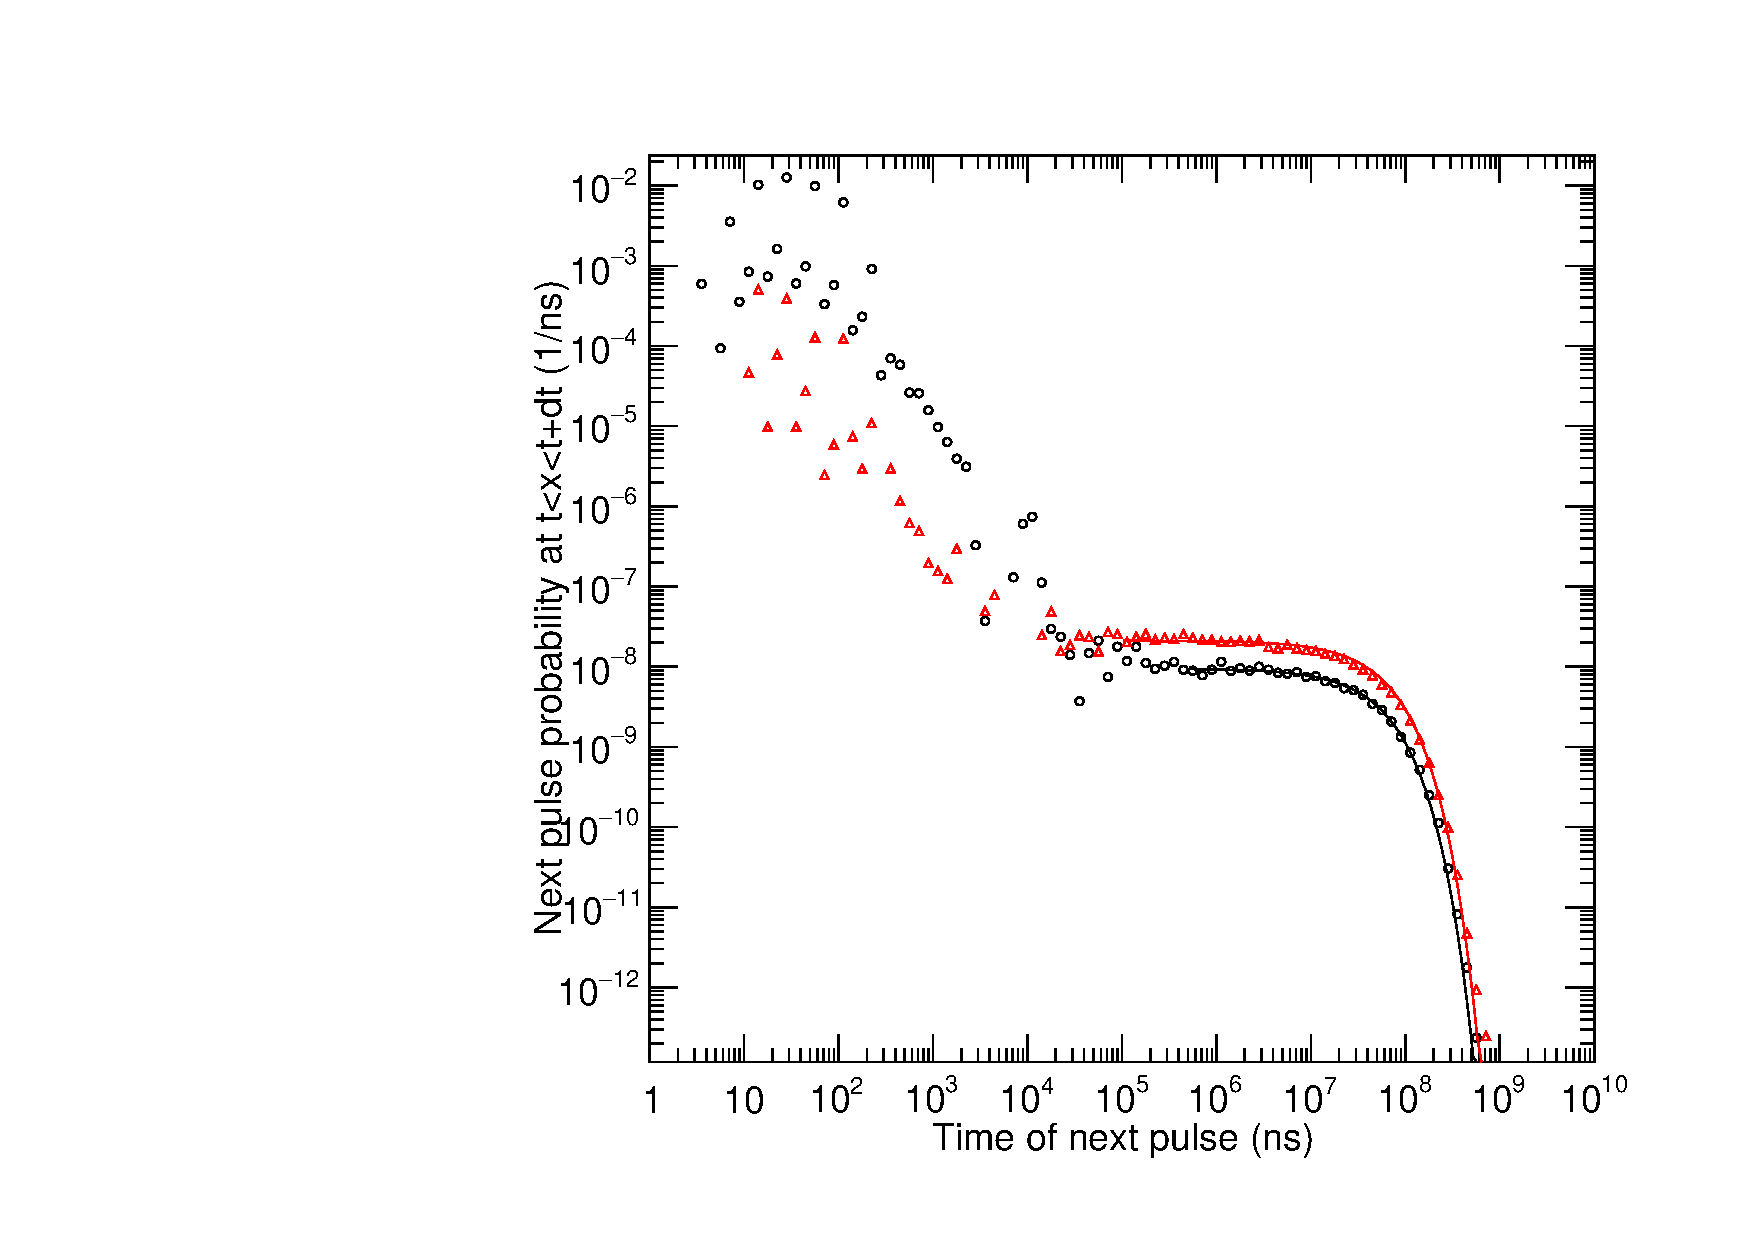
\includegraphics[height=0.5\textwidth]{DTVUV3.pdf}
\caption{Delta-time distribution for VUV3 device.}
\end{figure}
\end{frame}

\begin{frame}{Light Leak}
\begin{figure}
\centering
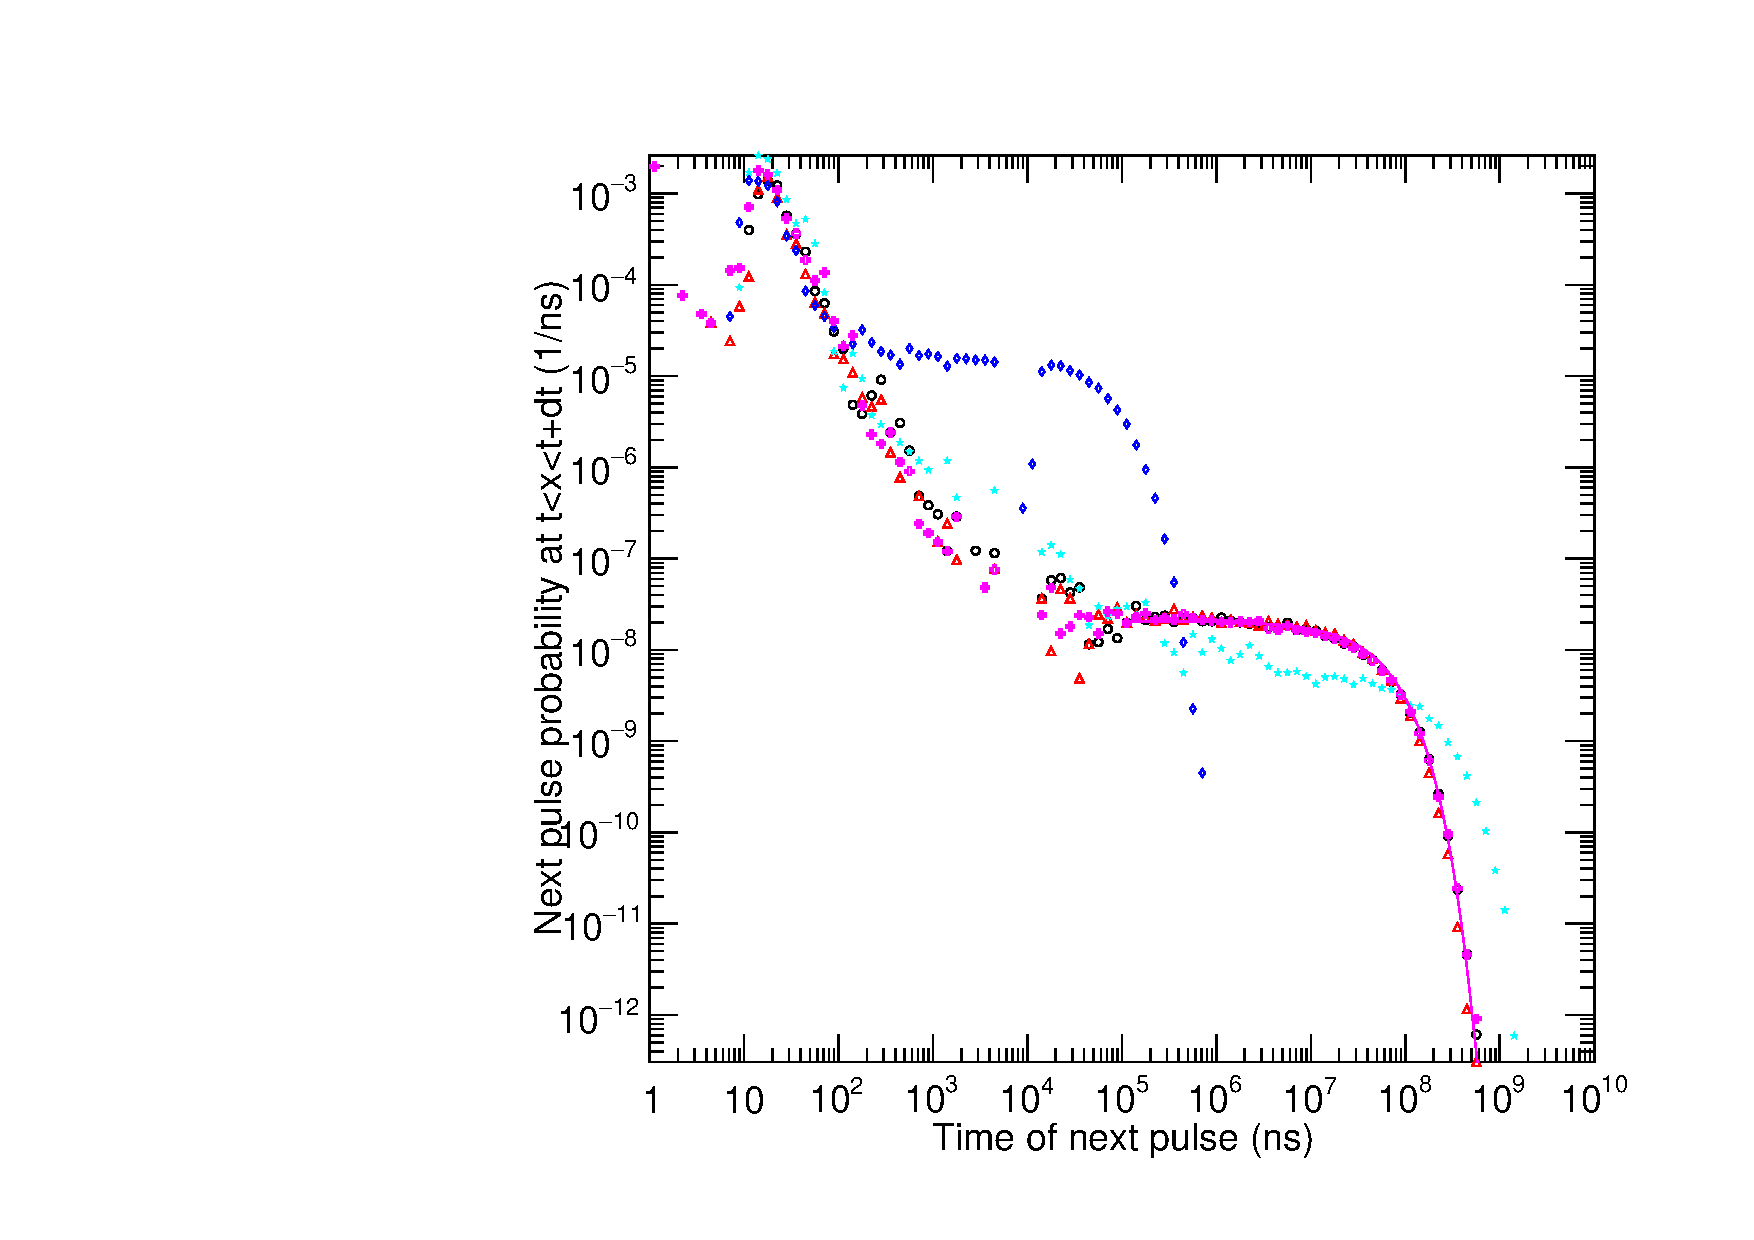
\includegraphics[height=0.5\textwidth]{DTimeLightLeakAug5.pdf}
\caption{Delta-time distribution showing that while there is light leak into the box, with the steps taken to cover the box there is no longer a leak.}
\end{figure}
\end{frame}

\begin{frame}{Troubleshooting}
To determine the source of the inconsistency in PE measurements, the following steps were taken:\\
\begin{itemize}
\item Installing temperature sensors in the setup to keep track of temperature at different places in the box.
\item Other stuff?
\end{itemize}
\end{frame}

\begin{frame}{Temperature Sensors}
\begin{figure}
\centering
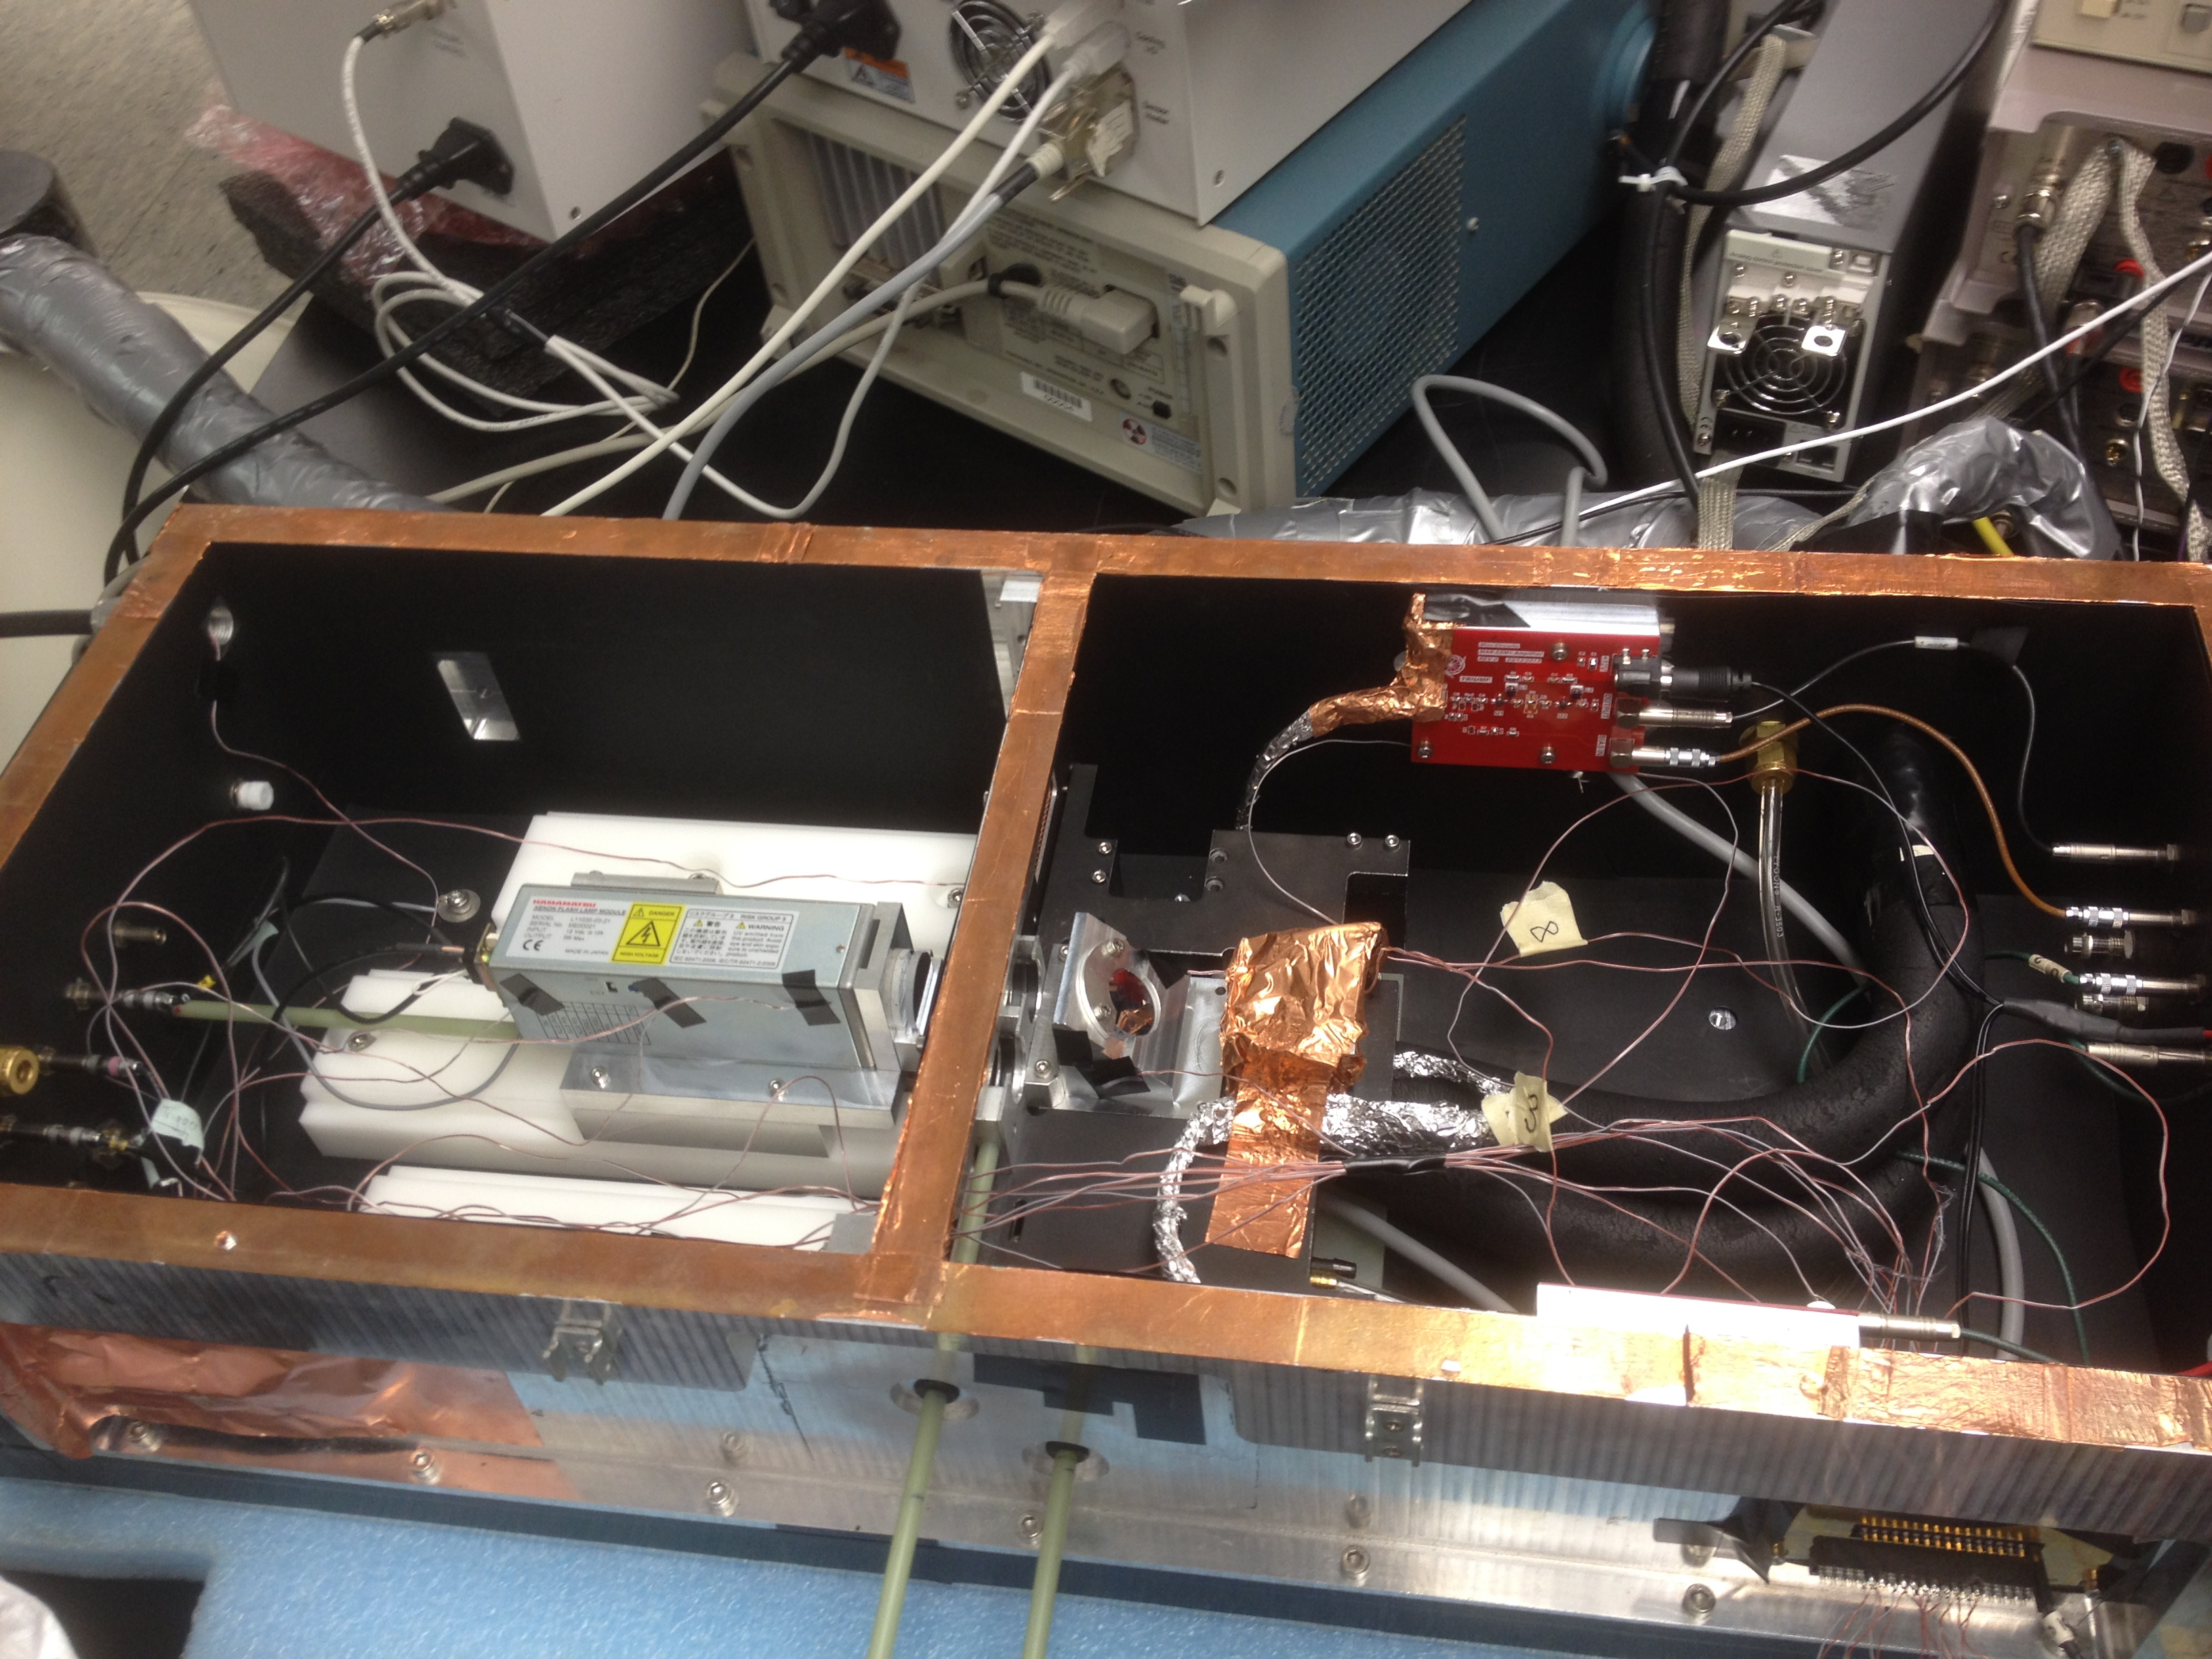
\includegraphics[height=0.5\textwidth]{sensors.JPG}
\caption{10 thermocouples were installed in various locations around the box so that temperature could be recorded in each location over time.}
\end{figure}
\end{frame}

\begin{frame}{Lamp Troubleshooting}
\begin{figure}
\centering
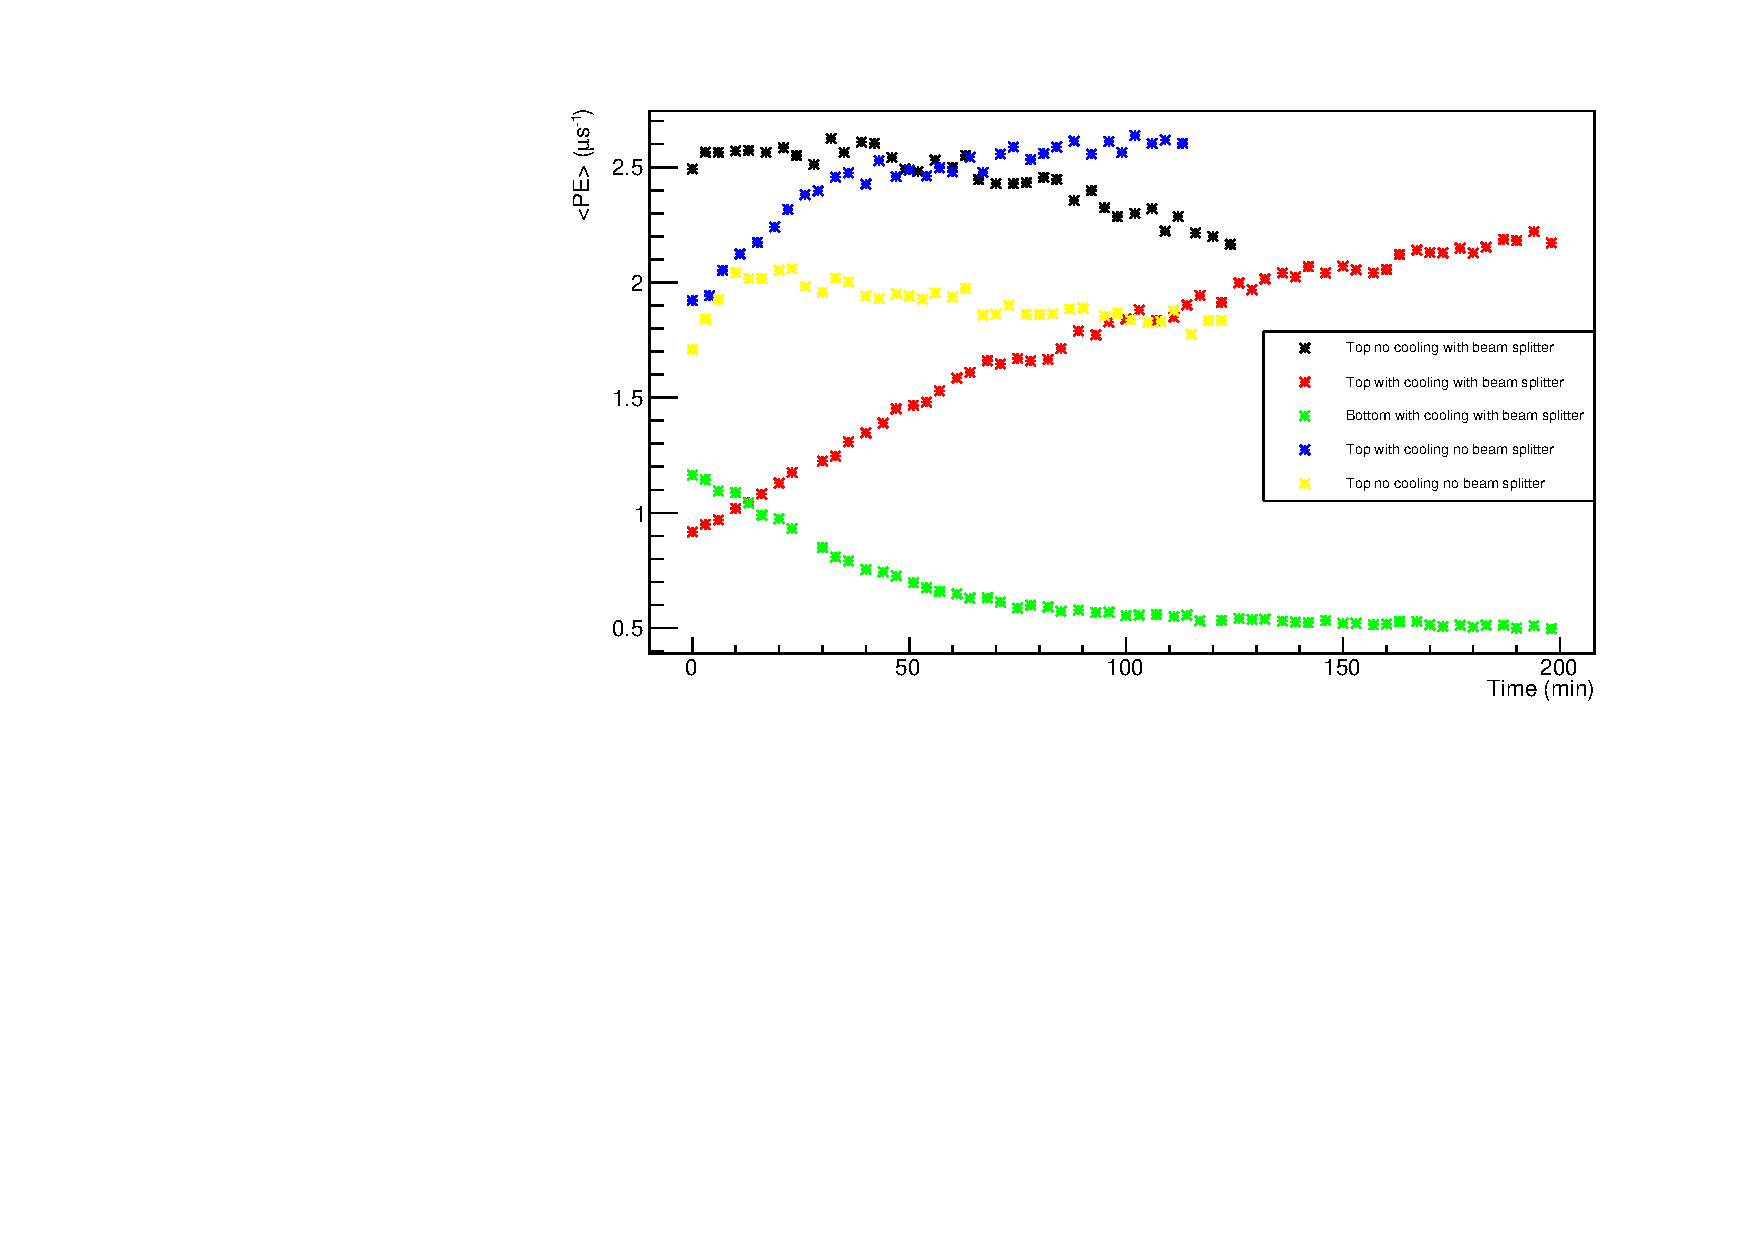
\includegraphics[height=0.5\textwidth]{NewLampPEAug5.pdf}
\caption{PE variation over 200 minutes in different cooling conditions.}
\end{figure}
\end{frame}

\begin{frame}{Lamp Troubleshooting}
\begin{figure}
\centering
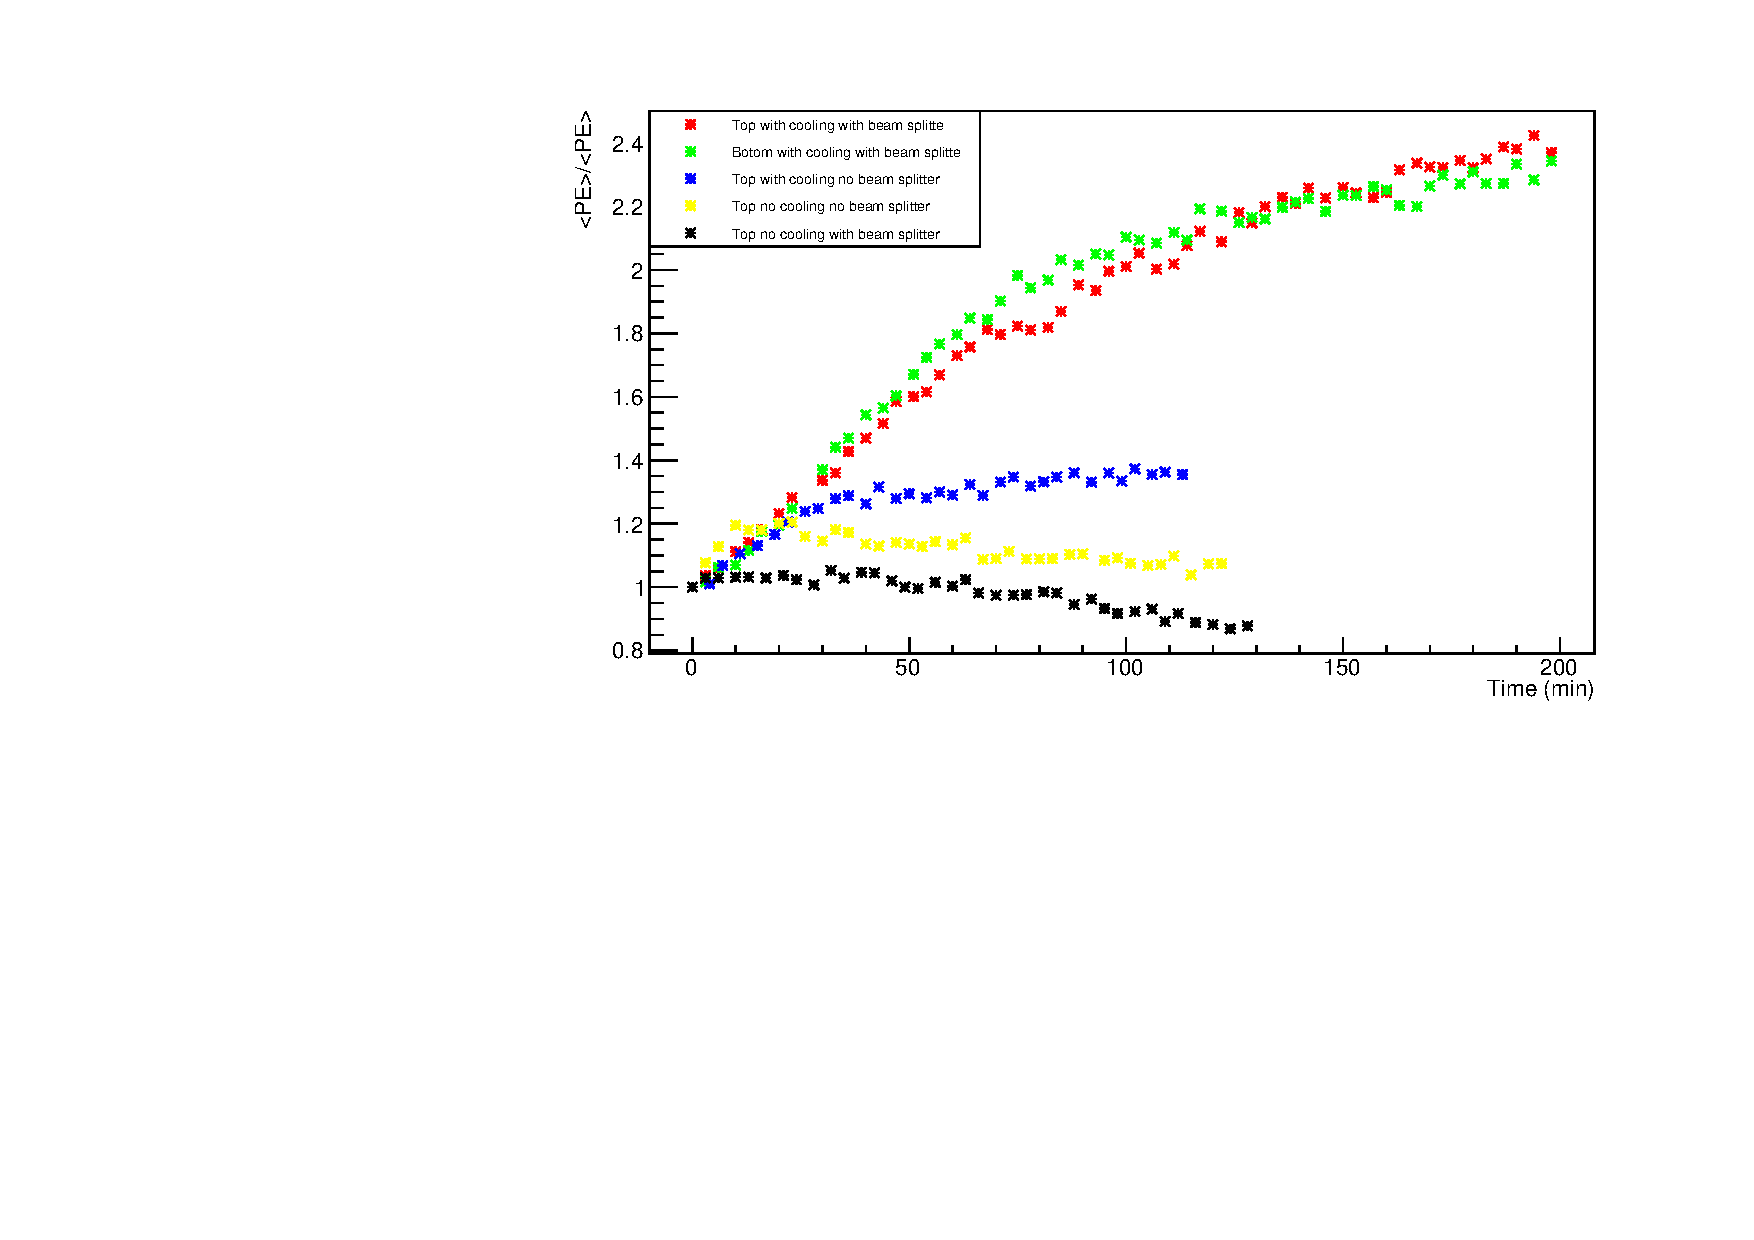
\includegraphics[height=0.5\textwidth]{NewLampPERatioAug5.pdf}
\caption{Variation of ratio of PE to initial PE over 200 minutes in different cooling conditions.}
\end{figure}
\end{frame}


\end{document}